\documentclass[../main.tex]{subfiles}
\begin{document}

\chapter[Transcriptome-wide association study of schizophrenia and 
chromatin activity]{Transcriptome-wide association study of 
	schizophrenia and chromatin activity yields mechanistic disease 
	insights}
\labch{gusev2018}

\extauth{Alexander Gusev, Nicholas Mancuso, Hyejung Won, Maria Kousi, 
Hilary K. Finucane, Yakir Reshef, Lingyun Song, Alexias Safi, 
Schizophrenia Working Group of the Psychiatric Genomics Consortium, 
Steven McCarroll, Benjamin M. Neale, Roel A. Ophoff, Michael C. 
O’Donovan, Gregory E. Crawford, Daniel H. Geschwind, Nicholas Katsanis, 
Patrick F. Sullivan, Bogdan Pasaniuc \& Alkes L. Price; Nature Genetics 
2018}

\begin{external_abstract}{title=Abstract}
Genome-wide association studies (GWAS) have identified over 100 risk 
loci for schizophrenia, but the causal mechanisms remain largely 
unknown. We performed a transcriptome-wide association study (TWAS) 
integrating a schizophrenia GWAS of 79,845 individuals from the 
Psychiatric Genomics Consortium with expression data from brain, blood, 
and adipose tissues across 3,693 primarily control individuals. We 
identified 157 TWAS-significant genes, of which 35 did not overlap a 
known GWAS locus. Of these 157 genes, 42 were associated with specific 
chromatin features measured in independent samples, thus highlighting 
potential regulatory targets for follow-up. Suppression of one 
identified susceptibility gene, mapk3, in zebrafish showed a significant 
effect on neurodevelopmental phenotypes. Expression and splicing from 
the brain captured most of the TWAS effect across all genes. This 
large-scale connection of associations to target genes, tissues, and 
regulatory features is an essential step in moving toward a mechanistic 
understanding of GWAS.
\end{external_abstract}

\section{Introduction}

GWAS hits are difficult to explain from a mechanistical point of view, 
for the association with the disease can arise in many different 
circumstances. In the great majority of cases, the GWAS hit is not even 
the real causal variant, but is merely in linkage disequilibrium with 
it; and even if we knew which is the actual causal variant, we still 
could not infer much about its functional role without a deeper 
knowledge of the biology at the locus where the variant lies. 
Integrating GWAS signals with a functional annotation of the genome can 
give insight into the mechanisms through which the variant affects the 
phenotype; in particular, it has been shown that schizophrenia GWAS hits 
were enriched in regulatory elements. In this paper, this concept was 
extended to transcriptome-wide association studies to identify putative 
regulatory mechanisms, through which the associations could make 
biological sense.

The regulatory role of a genetic region is mainly determined by its 
chromatinic state, \ie by how histones are modified, by which proteins 
bind in that region, and by whether the DNA is methylated or not; and 
its chromatinic state is in turn influenced by DNA elements either in 
\cis, for an alteration in a sequence that binds a protein can impair 
the protein's regulatory activity, or in \trans, for an altered protein 
that does not recognise a DNA motif any more cannot work properly. 
Ultimately, however, the chromatinic state of a region is under genetic 
control as much as any other phenotypic trait, therefore we have two 
effects that can spring from a genetic variant: the association with the 
disease or the association with the chromatinic state of a region. Such 
effects may or may not be independent. In this study the focus is on 
those genetic variants which both affect the chromatin structure of a 
locus, and alter gene expression, leading to a disease. The purpose, 
then, is to find a causal mechanism of action for variants associated 
with a disease.

The authors, by exploiting the method they had previously developed (see 
\refch{gusev2016}), performed a schizophrenia TWAS relying on 
summary-level data from a published large-scale GWAS, and subsequently 
performed a chromatin TWAS in order to find genes whose expression was 
associated with a chromatin phenotype. They then compared the two sets 
of genes aiming to gain insight into the biological function of the 
genes associated with schizophrenia. Their approach is summarised in 
\reffig{gusev2018/1}.

\begin{figure}
	\centering
	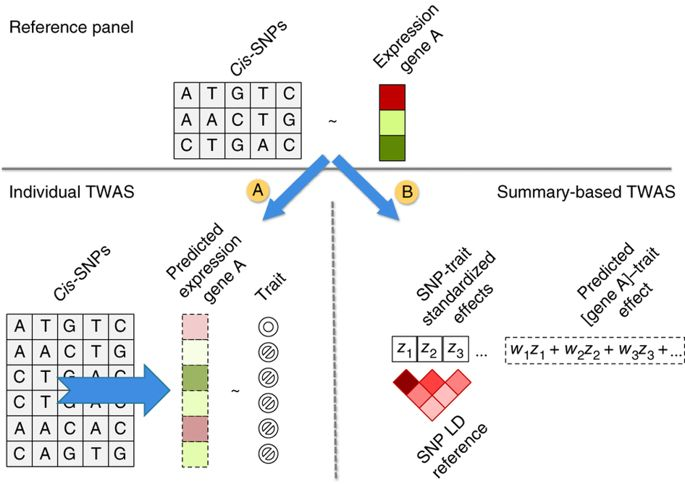
\includegraphics[width=0.55\textwidth]{gusev2018/1-TWAS_schematic}
	\labfig{gusev2018/1}
	\caption{The schematic of the TWAS approach used in the 
schizophrenia work.}
\end{figure}

\section{Schizophrenia}

Schizophrenia (MIM: \href{https://omim.org/entry/181500}{181500}), which 
affects more than 20 million people worldwide with symptoms such as 
hallucinations, delusions, depression, and poor cognitive functionality, 
is a psychiatric disorder characterised by a loss of contact with 
reality. As with any complex disease, the manifestation of schizophrenia 
is influenced both by genetic and by environmental factors; to date, 
more than 100 loci have been associated to this disease, and exposure to 
viruses, malnutrition or psychosocial factors are thought to have a 
contribution to it as well. Schizophrenia is treated with drugs and 
psychosocial support.

\section{Different levels of phenotype}
\labsec{phenolevels}

In this paper, the authors treated chromatin peaks as quantitative 
traits, much like they did with gene expression. This warrants further 
considerations on the nature of phenotypes.

The process of biological development of a multicellular organism is 
very complex: it involves signaling, differentiation, growth, cell 
division, and everything must happen in a coordinated fashion. The 
fascinating thing is that this process is self-regulated: the first cell 
contains all the information necessary to produce the final organism, 
and this information flows from moment to moment, from cell generation 
to cell generation, like a cascade carrying each cell towards its 
destiny. During development, all the genes interact with each other and 
contribute to the expression of phenotypes. No single gene can be held 
\textit{responsible} for a phenotype, but we can say that genetic 
differences at that gene in a population result in different 
phenotypes\autocite{Griffiths2000}. For example, a mutation in the gene 
\textit{white} of \textit{Drosohpila melanogaster} results in insects 
with white eyes instead of red; however, that gene just encodes for an 
ABC transporter\autocite{Mackenzie1999}, thus it cannot be responsible for 
the eye colour unless we insert it in the context of an already 
developed eye, which consists of many cells which assumed the structure 
of the eye during development. If we traced back the history of an eye 
cell, we would see that it changed dramatically, thanks to the 
collaboration of many genes; the \textit{white} gene is only the last 
one, and would not make sense without the previous history of the whole 
eye, and indeed of the whole organism.

Furthermore, DNA should not be seen as the only lowest-level determinant 
of every phenotype. Indeed, it is becoming clearer and clearer that 
epigenetic mechanisms can change gene expression (and other phenotypes 
as well) without altering DNA, and at the same time being inherited. 
This means that epigenetic mechanisms are under the effects of natural 
selection\autocite{Hunter2009}. But epigenetics is not the only high-level 
mechanism that can influence gene expression. When a cell undergoes 
mitosis or meiosis, each of the daughter cells stochastically inherits 
about half of the cytoplasm of the mother cell, and since the cytoplasm 
contains many molecules capable of altering gene expression ---such as 
transcription factors---, daughter cells are already \enquote{primed} 
towards a particular destiny, without any change to nucleotides. The 
fact that the cytoplasm can influence DNA can be clearly observed in 
cloning experiments, where embryogenesis is not triggered by the DNA 
itself, but by the cytoplasmic environment in which DNA lies.

Phenotypes can be seen at many levels: from chromatin states to gene 
expression, from the proteins present in the cell to eye colour, and 
even beyond the physical aggregate of cells which is the organism (for 
instance, a bird's nest is a phenotype, for a better nest increases the 
fitness of the bird, according to the view of the extended 
phenotype\autocite{Dawkins1999}). Any phenotype can, in principle, 
affect any other phenotype, as well as DNA itself (\eg some phenotypes 
increase mutation rate of DNA). Therefore, there is no linear 
relationship between genotype and phenotype, but rather a tight 
integration of all the levels. Evolution can act at different levels, 
too.

Genetic variation, however, can be argued to be the ultimate source of 
variation. Epigenetic modifications, for instance, need two pieces of 
DNA: a gene encoding for a DNA binding protein (or a 
methyl-transferase), and a sequence recognised and bound by the protein. 
According to what regions of DNA, be they coding or non-coding, are 
expressed, different enzymes and specific membrane transporters can be 
produced, thereby determining which reactions can happen and what 
molecules can enter the cell\autocite{Alberts2014}. Moreover, genetic 
variation is very easy to measure, so most efforts have concerned it.

\section{Traning of the expression models}

Coming back to the work of Gusev \etal, four datasets of either RNA-seq 
or genome-wide SNP-array expression measurements, for a total of nearly 
4,000 individuals,  were used to train the expression 
models\sidenote{RNA-seq from the dorsolateral prefrontal cortex of 621 
individuals (including 
283 schizophrenia cases, 47 bipolar cases, and 291 controls) collected 
	by the CommonMind Consortium (CMC); expression array data measured 
in peripheral blood from 1,245 unrelated control individuals from the 
Netherlands Twin Registry (NTR); expression array data measured in blood 
from 1,264 control individuals from the Young Finns Study (YFS); and 
RNA-seq data measured in adipose tissue from 563 control individuals 
from the Metabolic Syndrome in Men study (METSIM).}. In particular, some 
of the data came from the YFS and METSIM studies, and the weights for 
the SNPs in those cases were pre-computed by Gusev \etal for the 2016 
paper. The other dataset, the CMC, was added in order to train 
expression models in the brain, which is in all probability a relevant 
tissue in schizophrenia. The fact that both healthy individuals and 
patients were present in this last cohort did not impair the prediction 
of gene expression.

For each reference panel, \cis- and \trans- heritability of gene 
expression were computed and found significant for 18,084 genes (10,819 
unique). In addition, 9,009 splicing events in the brain were 
characterised, since an alteration of this kind of regulation is implied 
in disease. From such datasets, a sparse midex linear model (the BSLMM 
also used in the previous paper) was trained to find the weight of each 
\cis-SNP for each gene. Furthermore, since a population LD structure is 
necessary to estimate the correlation between the genetic component of 
expression and a phenotypic trait using summary GWAS information, LD 
informaton was also extracted from these data sets.

\section{Schizophrenia TWAS}

A separate TWAS was performed for each of the four reference gene 
expression training datasets, using the GWAS summary information from a 
large study of about 80,000 samples. 157 unique genes, of which 35 
completely novel (\ie being farther than 500kb from any previously 
associated SNP), were found significantly associated to the disease, as 
shown in \reffig{gusev2018/2}. Interestingly, 33 loci were found to 
harbour hotspots of multiple TWAS hits (\ie many genes less than 500kb 
apart), but, with a statistical test, it was found that in 27 of these 
cases the genes were correlated, suggesting a single underlying effect. 
For instance, this could be due to the alteration of the structure of an 
entire topologically associating domain (TAD).

\marginnote[-4cm]{For these analysis, the MHC region was not considered 
due to its complexity.}

\begin{figure}
	\centering
	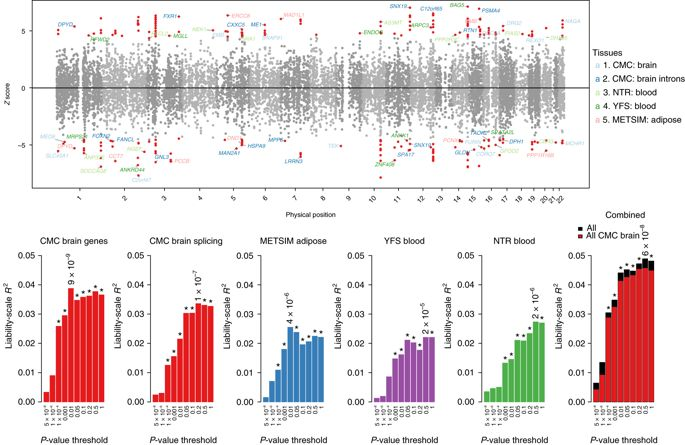
\includegraphics{gusev2018/2-schizophrenia_TWAS}
	\caption{Results of the schizophrenia TWAS. Red dots in the 
manhattan plot represent significant genes.}
	\labfig{gusev2018/2}
\end{figure}

Again, some evidence emerged that TWAS are more powerful than GWAS at 
detecting multiple variants whose combined effects explain the 
phenotype, rather than events where a single variant is involved (see 
\refsec{allelic_heterogeneity}): indeed, 27\% of the novel genes were 
associated to the disease more strongly than the top GWAS hit at the 
locus of the gene, whereas only 3\% of the genes overlapping a reported 
GWAS hit were more strongly associated than the GWAS hit 
(\reffig{gusev2018/S6}). This indicates that when there is a single 
causal variant, the GWAS is best at identifying it, but when there are 
multiple variants affecting the trait, the TWAS performs better.

\begin{marginfigure}
	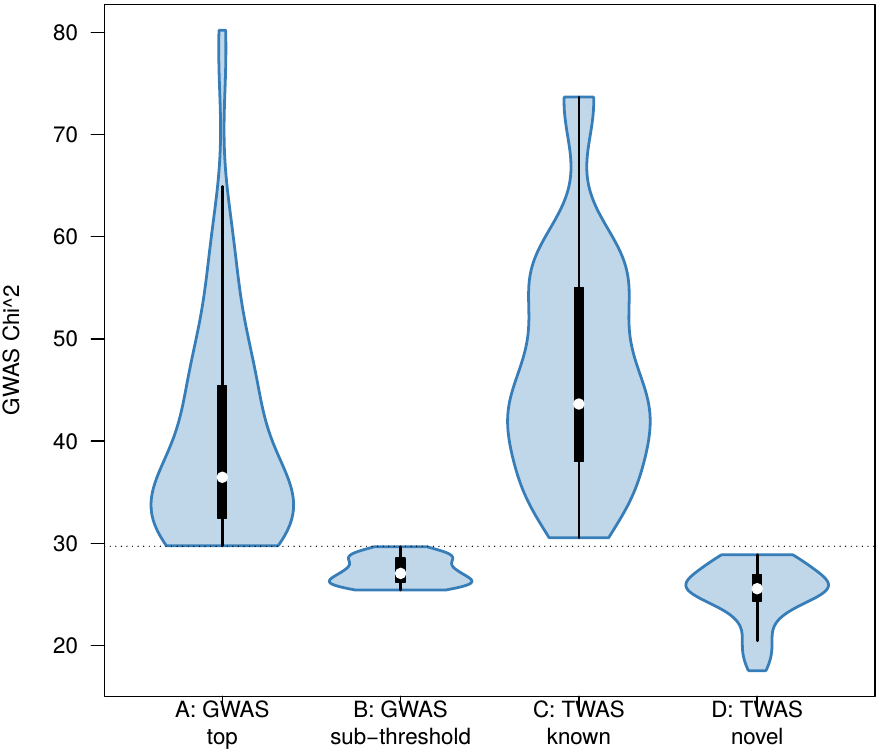
\includegraphics{gusev2018/S6-gwas_chi2}
	\caption{Violin plot of GWAS $\chi^2$ for different sets of 
variants.}
	\labfig{gusev2018/S6}
\end{marginfigure}

After finding those genes whose expression is associated to 
schizophrenia, the authors evaluated on the one hand whether there was 
an association between splicing events and disease, and on the other 
hand whether the significant genes had chromatin interactions with one 
of the causal SNPs associated to schizophrenia.

46 splicing events in the brain were also found associated to the 
   disease. Splice variants were detected using LeafCutter, a previously 
published algorithm which is based on the clustering of reads that span 
intron junctions; each cluster identify an isoform. The abundance of 
each isoform, after normalisation and PEER-correction, was treated as a 
quantitative trait in the same way as gene expression.

The chromatin interactions were derived from a Hi-C study of the human 
brain during development, while the causal SNPs were taken from the set 
of the fine-mapped ones\sidenote{Fine mapping aims to find the causal 
variants associated to a trait. First, all the SNPs in linkage 
disequilibrium with a GWAS hit are selected, then the probability of 
each variant to be causal is estimated with a difficult statistical 
method.}. From these data it was possible to trace back all the genes 
which physically interact with one of the causal SNPs. Among such 
\enquote{risk genes} there were 105 of the 157 TWAS-associated genes, 
pointing at a mechanistic reason for the associations and relating gene 
expression and regulation\sidenote{Actually, this mechanism is only 
valid if it is assumed to manifest during development, for the chromatin 
interaction experiment was performed in a zebrafish embryo.}.

\section{Chromatin TWAS}

Chromatin data for nine markers was obtained from 
ChIP-seq\sidenote{Chromatin immunoprecipitation-DNA sequencing consists 
in the sequencing of DNA fragments bound to specific proteins, captured 
by an antibody. In this case, the data came from lymphoblastoid cell 
lines from Yoruban and European populations:
\begin{description}
	\item[LCL of YRI:] acetylated histone H3 Lys27 (H3K27ac; marking 
active enhancers), methylated H3 Lys4 (H3K4me1; enhancers), 
trimethylated H3 Lys4 (H3K4me3; promoters), and DNase I–hypersensitive 
sites (DHS; open chromatin).
	\item[LCL of CEU:] H3K27ac, H3K4me1, H3K4me3, the regulatory 
transcription factor PU1, and RNA polymerase II (RPB2, associated with 
active transcription).
\end{description}
}, and the intensity of each peak was treated as a quantitative trait. 
Inside the cohorts with chromatin information, a TWAS was performed 
through the usual two steps: first, gene expression was imputed for the 
10,819 heritable genes and the spliced introns; then, gene expression 
and spliced introns expressionon was correlated to the chromatin state. 
Overall, 806 genes and 224 splicing events associated to at least one 
chromatin state were found (\reffig{gusev2018/3}).

\begin{figure}
	\centering
	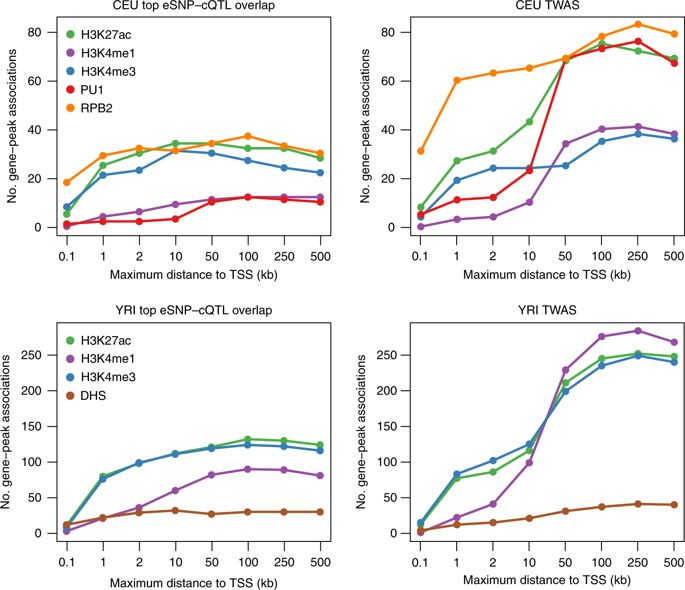
\includegraphics{gusev2018/3-chromatin_TWAS}
	\caption{Chromatin TWAS. eSNP-cQTL are those variants that influence 
both expression and chromatin, find by traditional analysis. The TWAS 
was able to find more associations, especially if the chromatin peak was 
far from the gene.}
	\labfig{gusev2018/3}
\end{figure}

\section{Putative regulatory mechanisms}

The integration of the two types of TWAS, that on chromatin and that on 
schizophrenia, can provide biological insight into the mechanism through 
which the associated genes influence the disease. Of the 157 genes 
associated to schizophrenia, 42 were also associated to a chromatin 
state, and, in particular, only 8 of the 42 genes were associated to a 
chromatin peak located in the promoter of the gene itself, suggesting 
that the majority of disease-associated genes are regulated by 
enhancers.

There are two possible models to explain the association between SNP and 
trait: one in which the SNP mediates the change in chromatin structure, 
which in turn alters gene expression leading to the disease; and one 
where the SNP directly mediates a change in the expression of some 
genes, and this in turn affects chromatin activity. In either case, the 
association of a gene both to a chromatin state and to a disease 
suggests the existence of particular regulatory mechanisms, which 
deserve experimental validation.

\section{Example}

As an example, the locus around the gene \textit{KLC1} was chosen. This 
gene encodes for the light chain of kinesin, which, as a tetramer 
composed of two heavy and two light chains, exploits microtubules to 
carry various molecules and other cargos along the cell 
(\reffig{gusev2018/kinesin}). \reffig{gusev2018/5} shows in (a) an 
overview of the locus: the gene is associated to schizophrenia and to 
two chromatin peaks ---H3K4me1 and H3K4me3---, and an Hi-C signal 
confirms the interaction between the promoter of \textit{KLC1} and the 
regions where the chromatin peaks lie. The other portion of the figure, 
(b), display on the left a manhattan plot of the P-values of association 
between SNP and disease status, with the association either being 
weighted for the expression (coloured dots, like in a TWAS) or not 
(black dots, like in a GWAS); on the right, there are scatter plots 
reporting on the $y$ axis the z-score of the association between GWAS 
and eQTL, and on the $x$ axis the correlation between the z-score and 
the predicted expression.

\begin{marginfigure}[-4.5cm]
	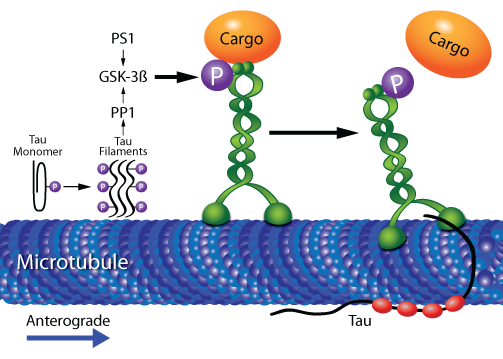
\includegraphics{gusev2018/ext-kinesin}
	\caption{A kinase phosphorilates the kinesin triggering a 
conformation change in the protein which results in its movement along 
the microtubule filament. \url{https://www.cytoskeleton.com}}
	\labfig{gusev2018/kinesin}
\end{marginfigure}

\begin{figure}
	\centering
	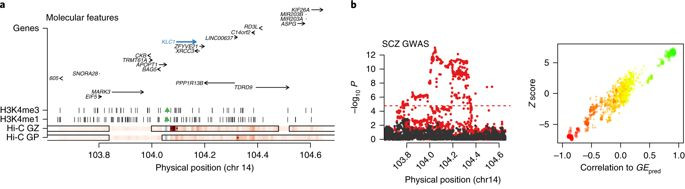
\includegraphics{gusev2018/5-KLC1}
	\caption{the \textit{KLC1} locus.}
	\labfig{gusev2018/5}
\end{figure}

It can be seen from (b) that no SNP was genome-wide significant at that 
locus, but after accounting for their contribute to gene expression, 
many of the variants passed the significancy threshold and were 
therefore transcriptome-wide significant. Finally, the relationship 
between the z-score and the predicted expression is linear and has a 
positive slope, meaning that the more the gene is expressed, the higher 
the risk to develop schizophrenia.

\section{Functional validation}

Another interesting gene whose expression correlated with schizophrenia 
and with two chromatin peaks, is \textit{MAPK3}, encoding a 
mitogen-activated protein kinase which regulates many aspects of cell 
growth and proliferation. 

Previous studies found that \textit{MAPK3} and \textit{KCTD13} are 
coregulated, and that \textit{KCTD13} over-expression causes 
microcephaly because of its impairment of neuronal proliferation. The 
TWAS results show that if \textit{MAPK3} is over-expressed, then the 
risk of disease increases; the authors hypothesised that, if 
\textit{MAPK3} acts through \textit{KCTD13} on schizophrenia, then 
down-regulating the gene should rescue the disease.

A zebrafish model over-expressing \textit{KCTD13} was built to test this 
hypothesis (\reffig{gusev2018/6}). As expected, the heads of the fish 
embryos were small and the cells therein were less proliferative, but 
after the suppression of \textit{MAPK3}, the embryos developed normally.

\begin{figure}
	\centering
	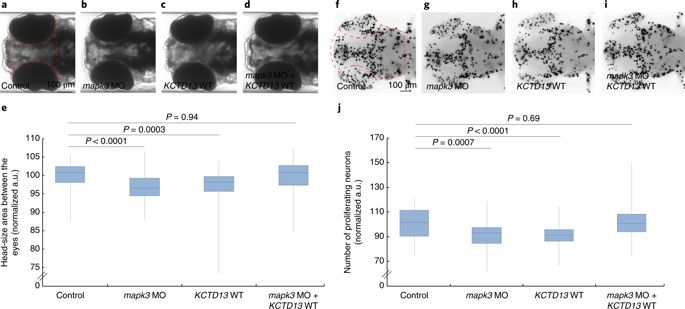
\includegraphics{gusev2018/6-zebrafish}
	\caption{A zebrafish model validates the discovery of a gene 
associated to schizophrenia.}
	\labfig{gusev2018/6}
\end{figure}

It could be argued that this is not a real validation, for fish do not 
have schizophrenia. However, modeling human psychiatric disorders is not 
easy either. At least, this experiment validates that the gene and the 
phenotype are indeed associated, even in the real world.

\section{Discussion}

The motivation behind this work was double: first, an association does 
not imply a causal mechanism; secondly, gene expression is not the only 
way through which genetic variants can alter a phenotype. For instance, 
a gene can be differentially spliced without its expression level 
changing.

This was also an attempt to go beyond genetic variants alone and relate 
chromatin structure to gene expression. The integration of a disease 
TWAS with a chromatin activity TWAS allowed to make hypothesis on the 
mechanism through which the expression is regulated. A direct 
association between chromatin activity and disease, however, was never 
proven\sidenote{Indeed, the sample size was too small to perform a 
chromatin-wide association study}, therefore these result provide 
possible mechanistic explainations for how genetic variants regulate 
gene expression through the modification of chromatin (or \textit{vice 
versa}), and not for how the altered expression of a gene lead to the 
disease.

The method and most of the data set where the expression models were 
trained, were the same as those used in the previous article. A new 
entry here was the integration of experimental biology to suggest or 
validate hypothesis. First, the chromatin interactions were used to 
confirm that, at least once in the life of a living organism, 
disease-associated genes interacted with disease-associated SNPs. Then a 
zebrafish model validated an hypothesis on a particular gene, 
\textit{MAPK3}.

\end{document}
